\documentclass[11pt, a4paper, twocolumn]{article}
\usepackage[utf8]{inputenc}
\usepackage{url}
\usepackage{hyperref}
\usepackage[margin=1.5cm]{geometry}
\usepackage{graphicx}
\usepackage{amsmath}
\usepackage{amssymb}
\usepackage{booktabs}
\usepackage{array}
\usepackage{float}


\title{
\begin{flushleft}
\includegraphics[width=3.5cm]{images/uibknew.eps}
\hfill
\includegraphics[width=1.8cm]{images/igslogo.png}
\hspace{0.3cm}
\includegraphics[width=0.9cm]{images/iislogo.png}
\end{flushleft}\vspace{0.5cm}
Visual Computing Project Report}
\author{Tim Dedie \& Nick Somitsch}

\begin{document}


\maketitle

\thispagestyle{empty}


\section*{Introduction}
\textbf{Task.} We built a system that recognizes hand gestures from a webcam feed. It classifies five gestures: thumbs up, thumbs down, peace sign, open palm, and no hand (Figure~\ref{fig:gestures}).

\begin{figure}[H]
    \centering
    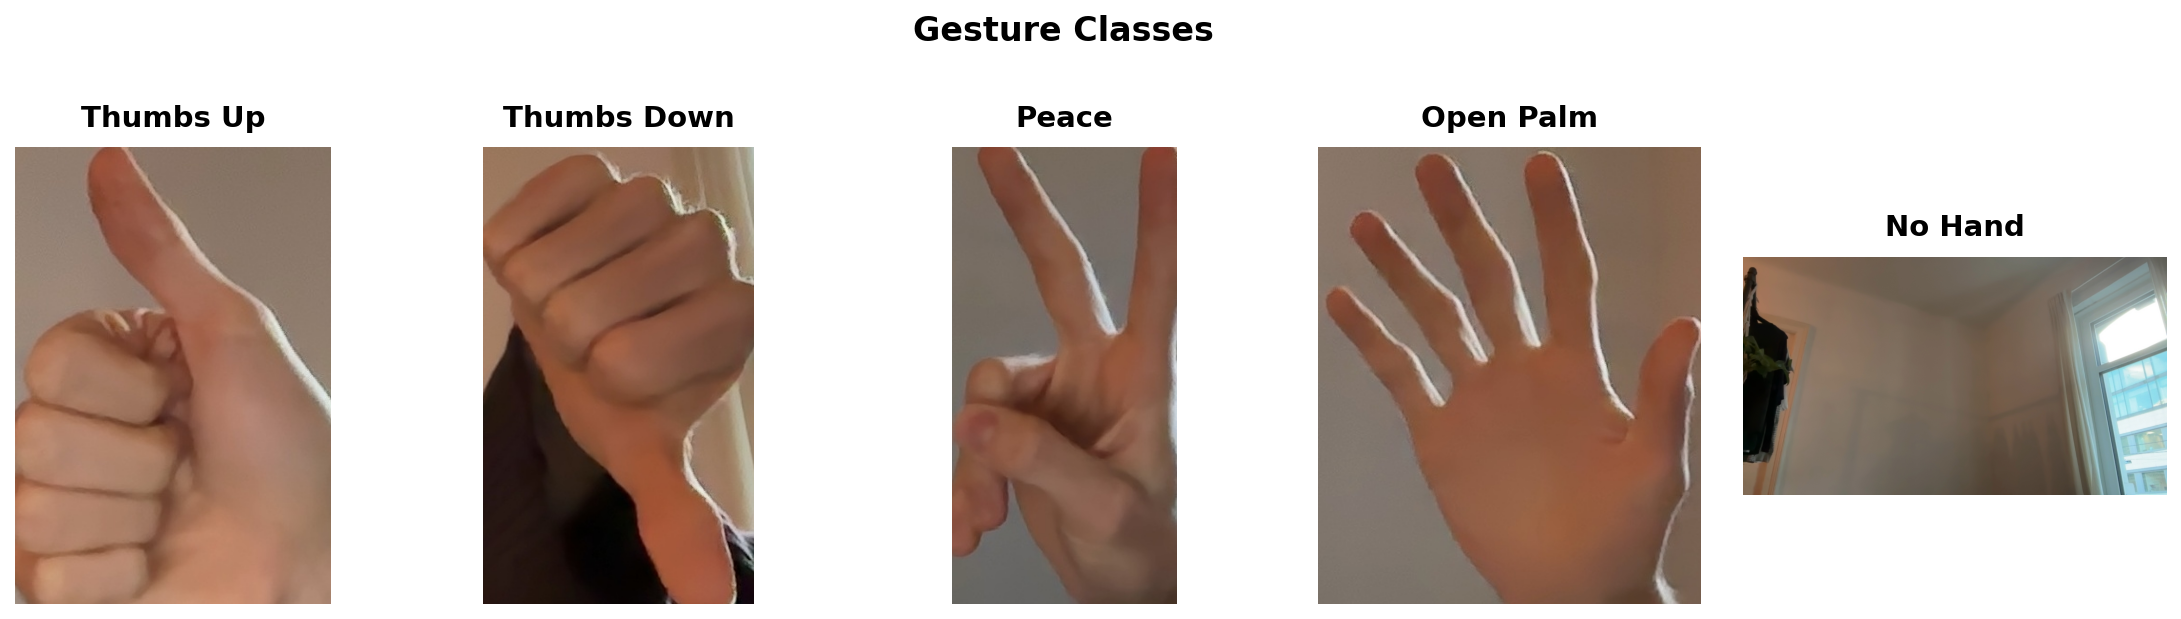
\includegraphics[width=\columnwidth]{images/gesture_samples.png}
    \caption{The five gesture classes our system recognizes.}
    \label{fig:gestures}
\end{figure}

\textbf{Problem.} Our first attempts didn't work well. We fed full webcam frames into the network and the model just learned to recognize the background instead of the actual hand gestures. If we recorded thumbs up in front of a bookshelf, the model associated "bookshelf" with thumbs up. This was frustrating until we realized we needed to crop out just the hand first.

\textbf{Solution.} We use Google's MediaPipe to detect and crop the hand region, then feed that cropped image to a CNN for classification. With this approach and the right augmentation settings, we got 100\% accuracy on our test set.

\textbf{Contributions.} Tim: data collection and augmentation experiments. Nick: CNN implementation, training scripts, and live demo.

\section*{Background}
\textbf{Why MediaPipe?} MediaPipe Hands is a pre-trained model from Google that detects 21 landmarks on a hand (fingertips, knuckles, palm, etc.). We use these points to draw a bounding box around the hand and crop it out. This way our CNN only sees the hand, not the background.

\textbf{Our CNN architecture.} We use a simple CNN with three convolutional blocks:
\begin{itemize}
    \item Input: $64 \times 64$ RGB image (3 channels)
    \item Conv1: 3 $\rightarrow$ 32 filters, $3\times3$ kernel, ReLU, MaxPool $\rightarrow$ output $32 \times 32$
    \item Conv2: 32 $\rightarrow$ 64 filters, $3\times3$ kernel, ReLU, MaxPool $\rightarrow$ output $16 \times 16$
    \item Conv3: 64 $\rightarrow$ 128 filters, $3\times3$ kernel, ReLU, MaxPool $\rightarrow$ output $8 \times 8$
    \item Flatten: $128 \times 8 \times 8 = 8192$ features
    \item FC1: 8192 $\rightarrow$ 256, ReLU, Dropout (50\%)
    \item FC2: 256 $\rightarrow$ 5 (one per gesture class)
\end{itemize}
Total: about 2.19 million parameters. Figure~\ref{fig:architecture} shows the full architecture.

\begin{figure}[H]
    \centering
    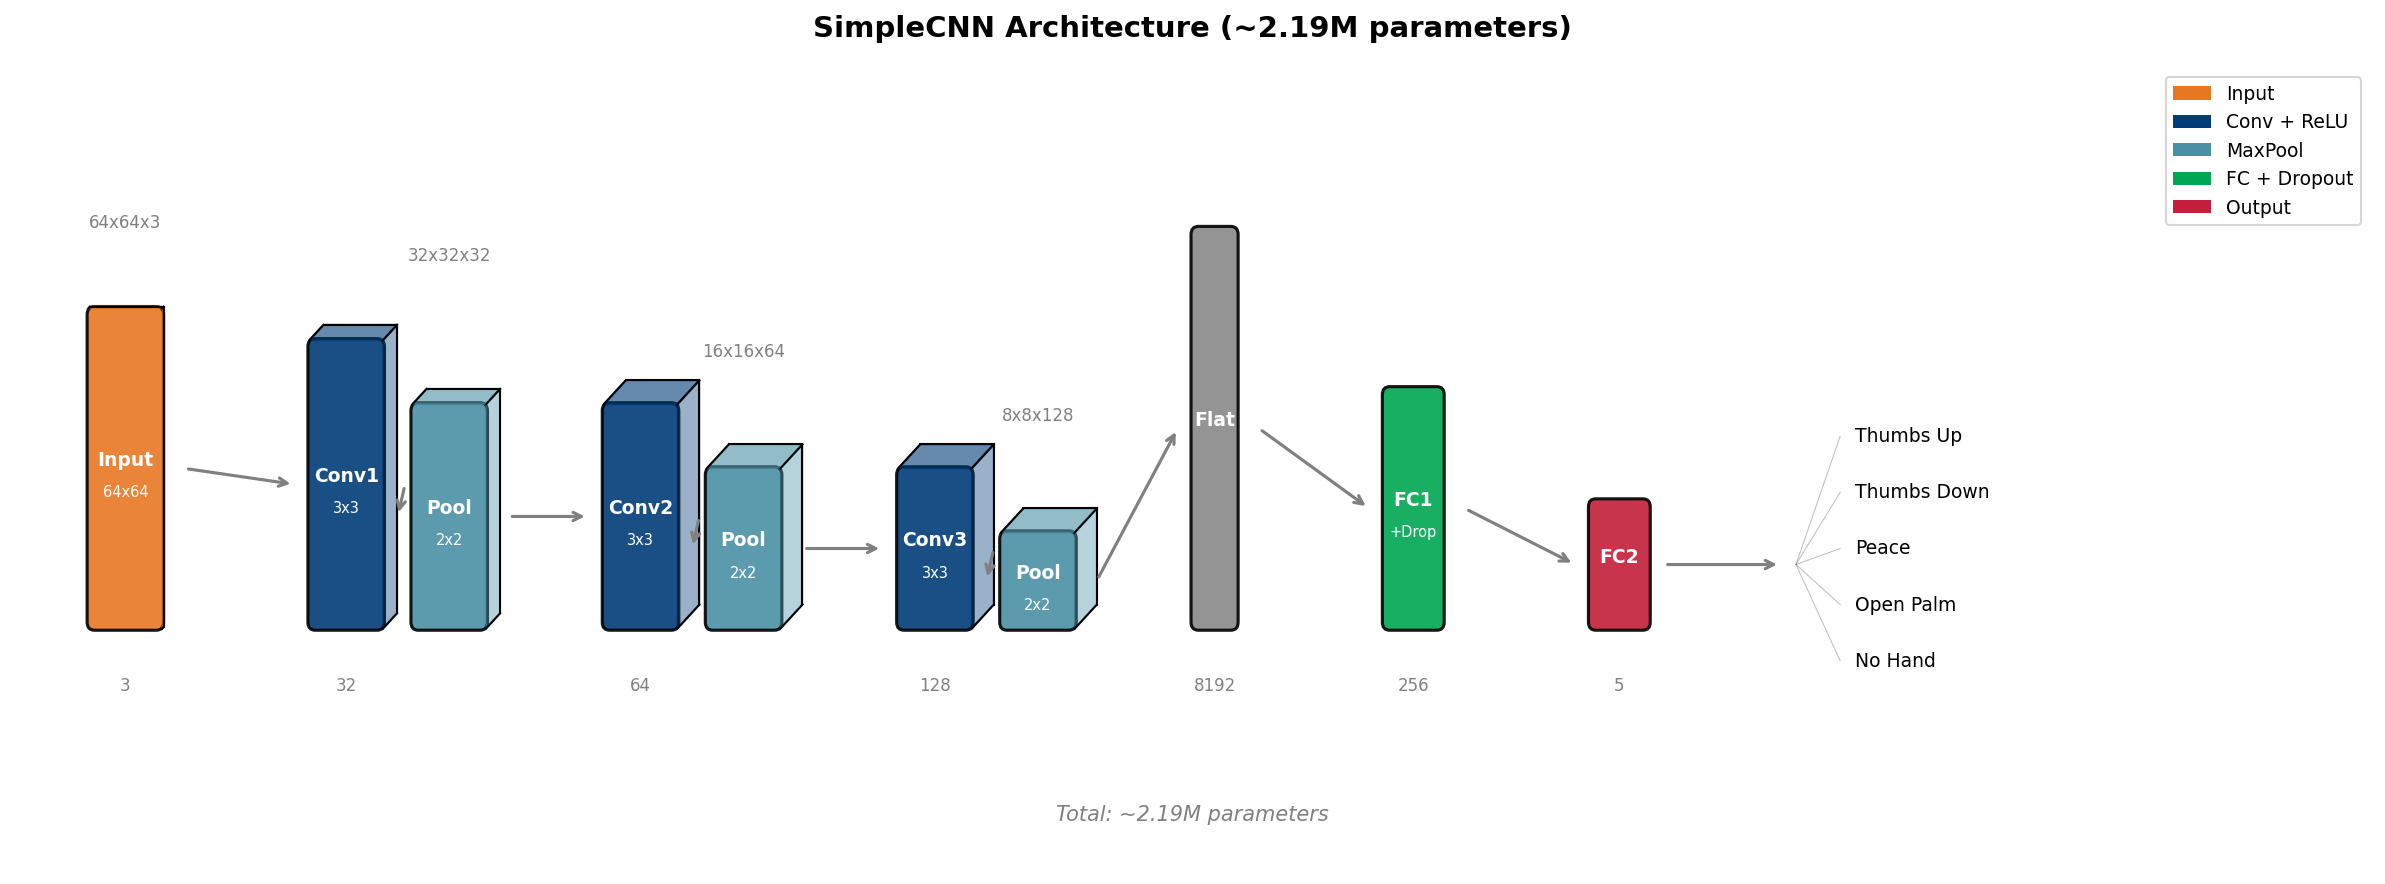
\includegraphics[width=\columnwidth]{images/architecture.png}
    \caption{Our SimpleCNN architecture.}
    \label{fig:architecture}
\end{figure}

\textbf{Loss function.} We use softmax and cross-entropy:
\begin{align}
    p_i = \frac{\exp(z_i)}{\sum_j \exp(z_j)}, \quad
    \mathcal{L} = -\sum_i y_i \log p_i
\end{align}

\textbf{Augmentations.} We implemented these ourselves with OpenCV (no torchvision):
\begin{itemize}
    \item Horizontal flip -- mirrors the image
    \item Rotation -- random angle between $-30°$ and $+30°$
    \item Brightness -- multiply by random factor 0.5 to 1.5
    \item Gaussian blur -- kernel size 3, 5, or 7
    \item Color jitter -- shift hue and saturation in HSV
    \item Zoom -- scale up and crop center
\end{itemize}
Each augmentation is applied with 50\% probability during training. Figure~\ref{fig:augmentations} shows examples of each augmentation applied to the same image.

\begin{figure}[H]
    \centering
    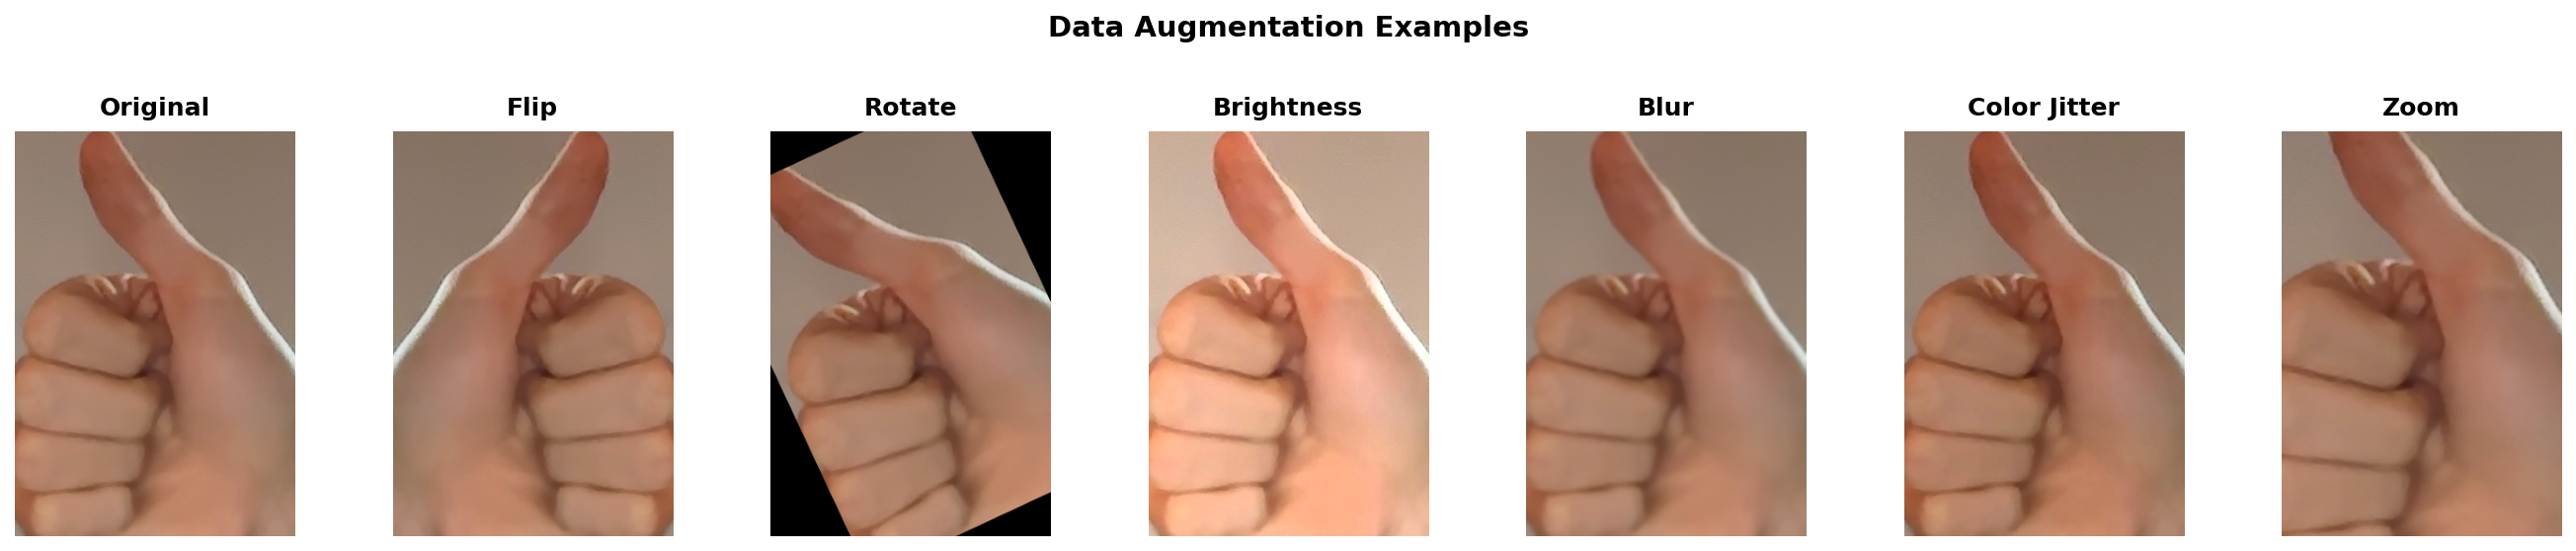
\includegraphics[width=\columnwidth]{images/augmentation_examples.png}
    \caption{Examples of our data augmentations.}
    \label{fig:augmentations}
\end{figure}

\section*{Method}
Figure~\ref{fig:pipeline} shows our complete pipeline from webcam input to gesture classification.

\begin{figure}[H]
    \centering
    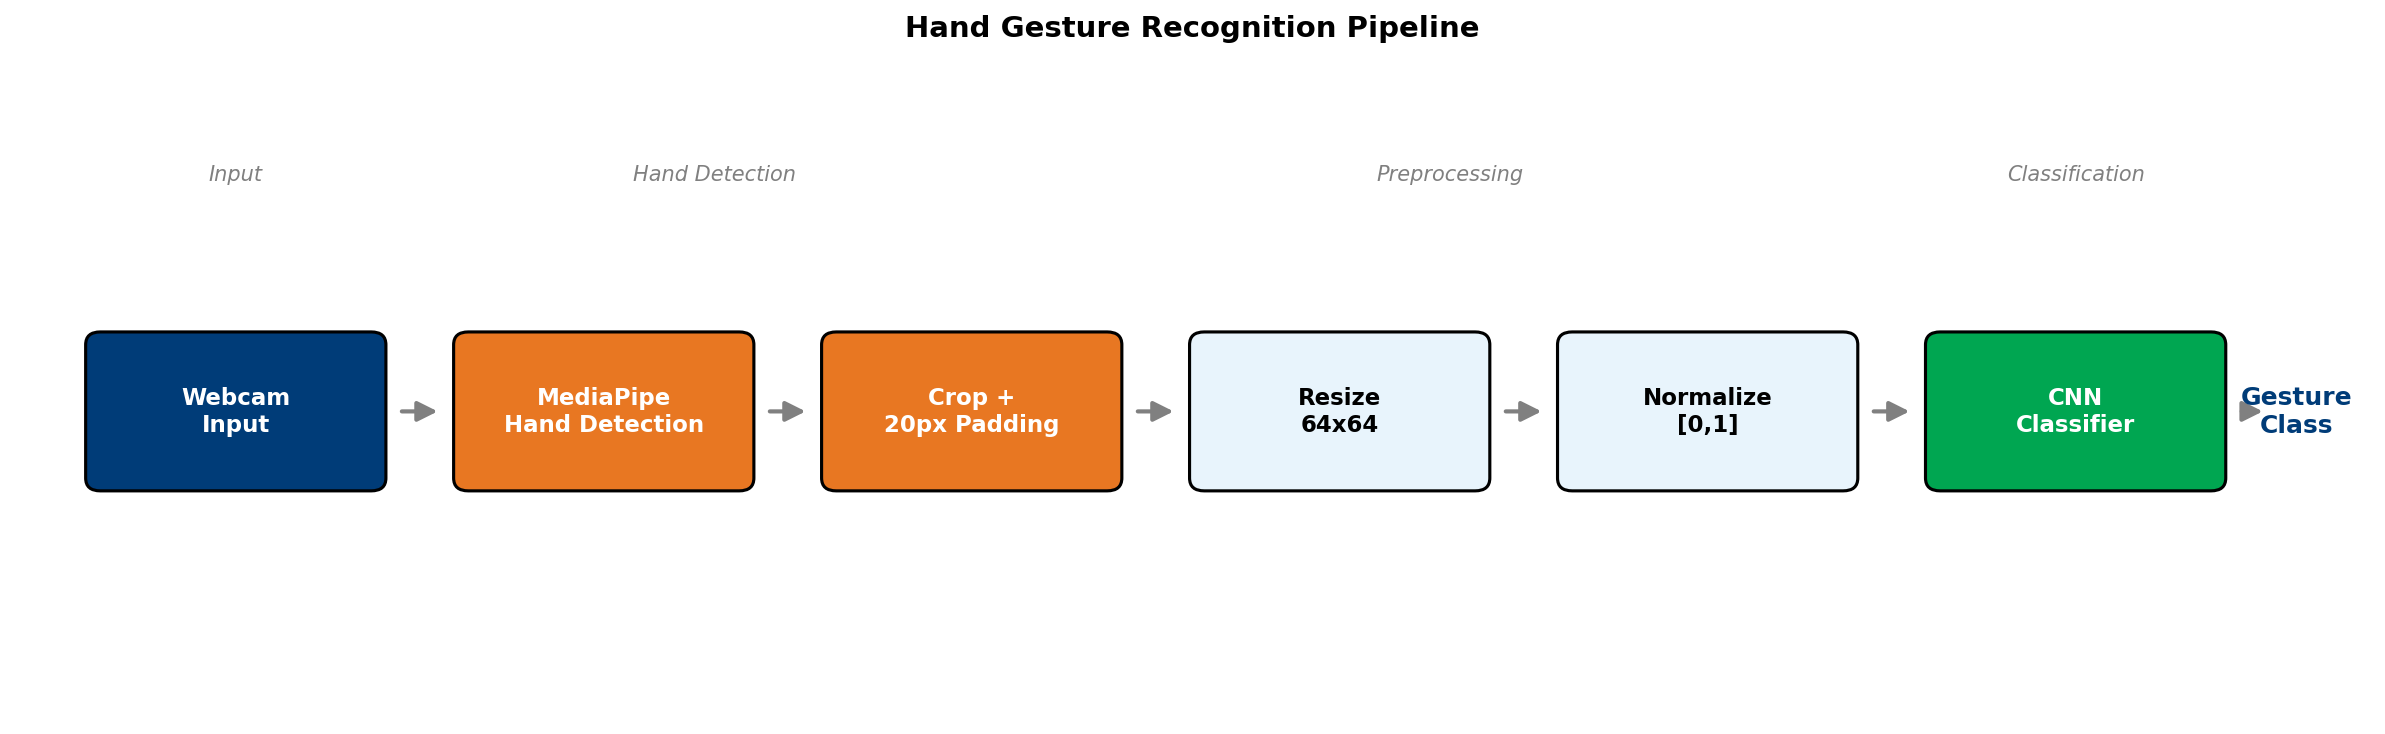
\includegraphics[width=\columnwidth]{images/pipeline.png}
    \caption{Our hand gesture recognition pipeline.}
    \label{fig:pipeline}
\end{figure}

\textbf{Data collection.} We wrote a script that:
\begin{enumerate}
    \item Captures webcam frames
    \item Runs MediaPipe to find the hand
    \item Crops the hand region with 20px padding
    \item Saves to folders (one per gesture class)
\end{enumerate}
We collected around 300 images per class. For "no hand" we just saved the full frame.

\textbf{Preprocessing pipeline:}
\begin{enumerate}
    \item Load image with OpenCV
    \item Apply augmentation (50\% chance, training only)
    \item Resize to $64 \times 64$
    \item Normalize to $[0, 1]$
    \item Convert from HWC to CHW format
\end{enumerate}

\textbf{Training setup:}
\begin{itemize}
    \item Optimizer: Adam, learning rate 0.001
    \item Loss: CrossEntropyLoss
    \item Epochs: 20
    \item Batch size: 32
    \item Train/test split: 80/20, stratified, seed 42
\end{itemize}
Figure~\ref{fig:training_curves} shows how the models learn over time. All configurations converge within 20 epochs.

\begin{figure}[H]
    \centering
    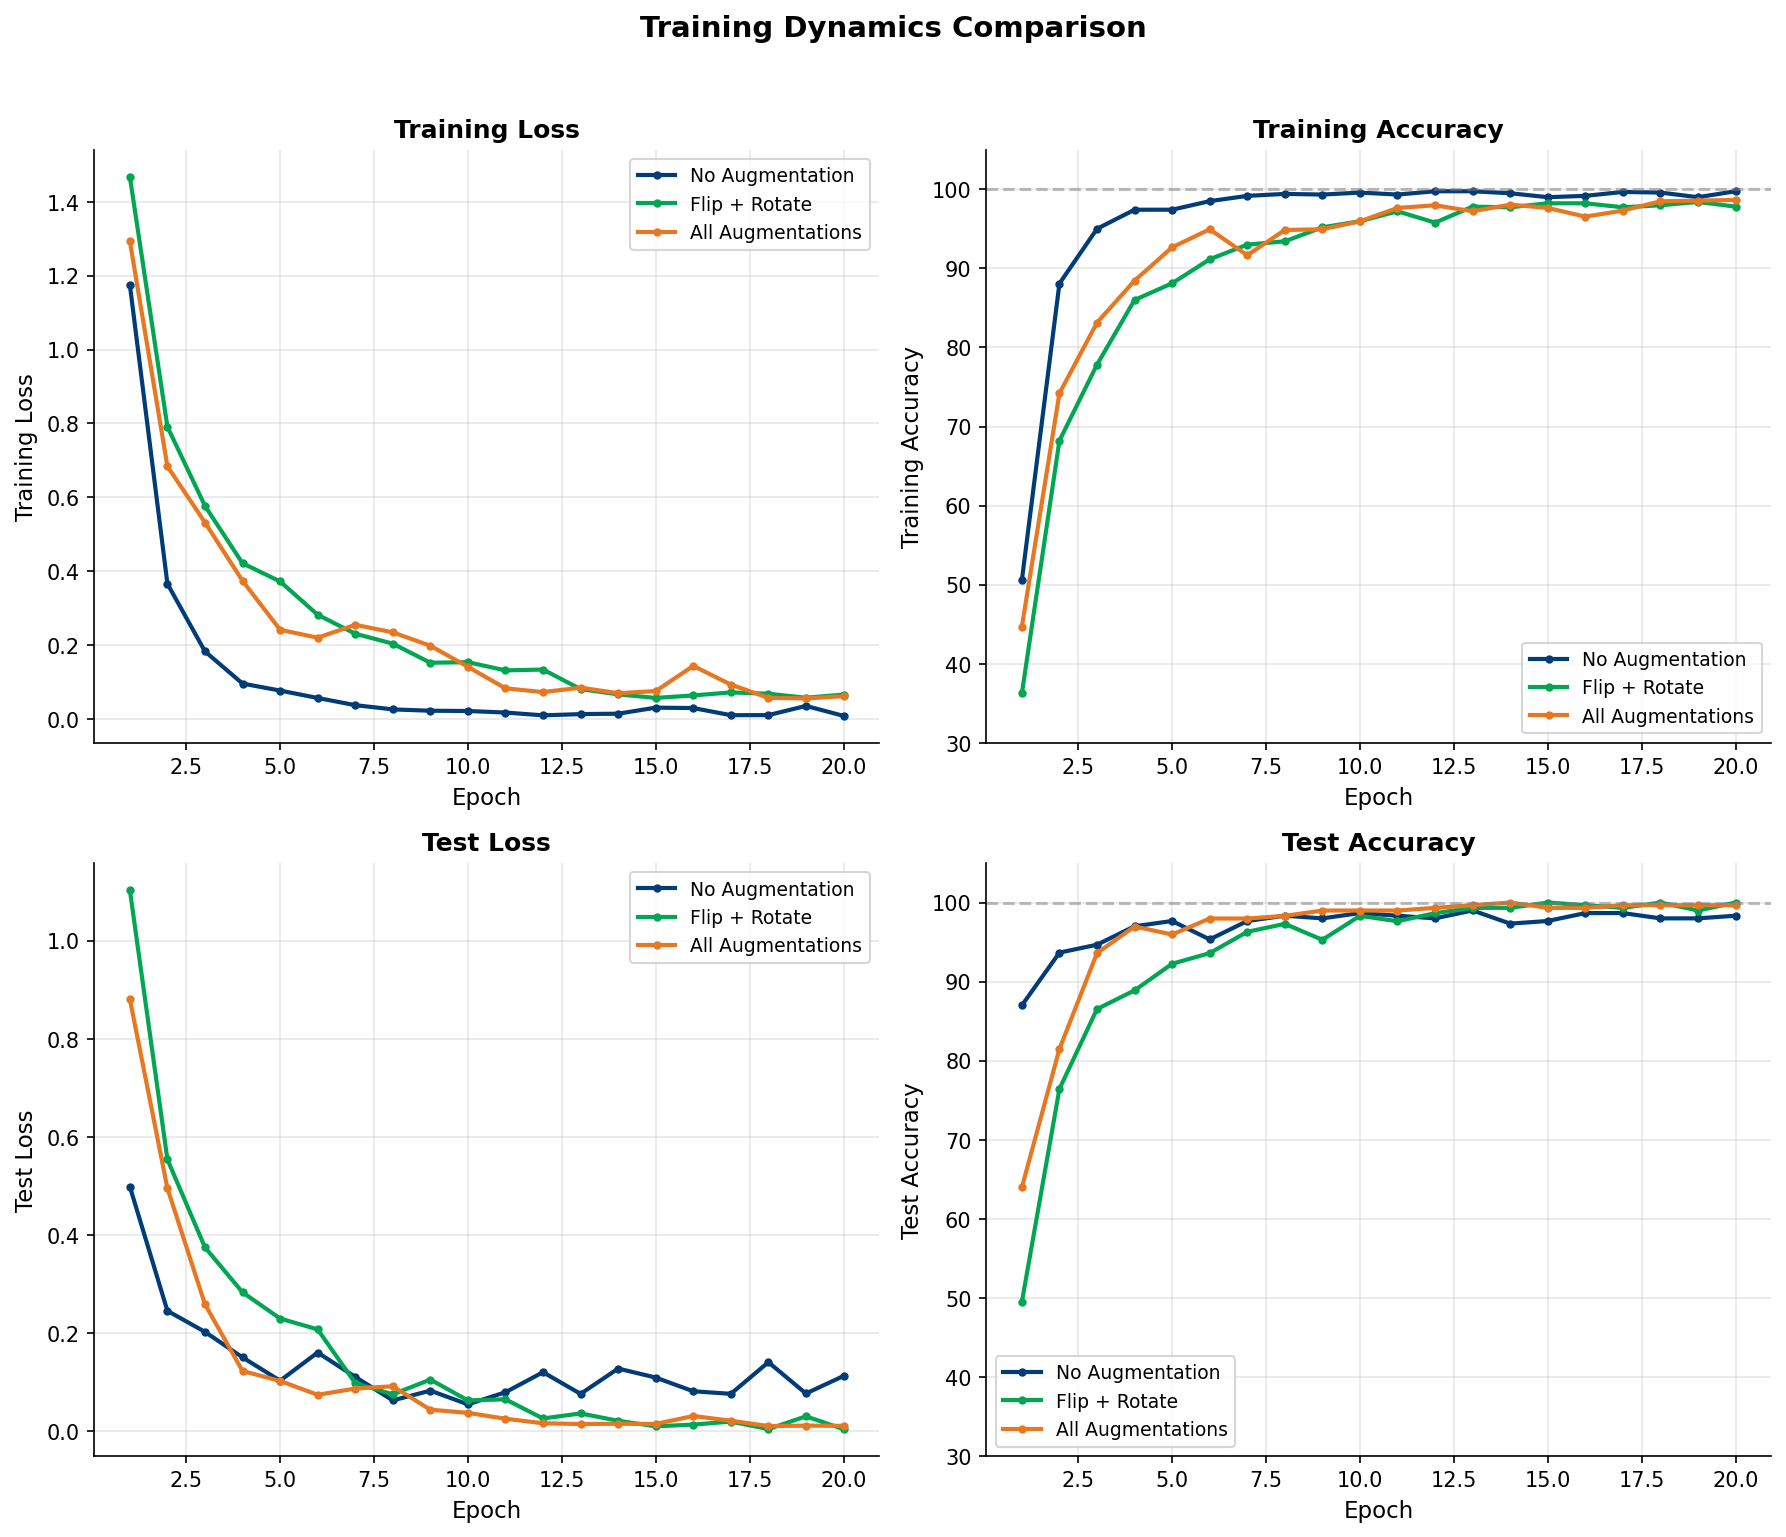
\includegraphics[width=\columnwidth]{images/training_curves.png}
    \caption{Training and test loss/accuracy over 20 epochs.}
    \label{fig:training_curves}
\end{figure}

\textbf{Experiments.} We ran two sets of experiments:
\begin{enumerate}
    \item \textit{Augmentation comparison}: no augmentation, single augmentations (flip, rotate, brightness, blur), flip+rotate combined, all augmentations
    \item \textit{Dataset size}: 50, 100, 200, and full samples per class, with and without augmentation
\end{enumerate}

\section*{Results}
\textbf{Augmentation results.} Table~\ref{tab:augmentation} and Figure~\ref{fig:aug_comparison} show that flip+rotate gives the best results -- even better than using all augmentations together.

\begin{table}[H]
\centering
\caption{Test accuracy by augmentation}
\label{tab:augmentation}
\begin{tabular}{@{}lc@{}}
\toprule
Config & Accuracy \\
\midrule
None & 98.33\% \\
Flip only & 96.33\% \\
Rotate only & 97.67\% \\
Brightness only & 98.00\% \\
Blur only & 98.67\% \\
Flip + Rotate & \textbf{100.00\%} \\
All & 99.67\% \\
\bottomrule
\end{tabular}
\end{table}

\begin{figure}[H]
    \centering
    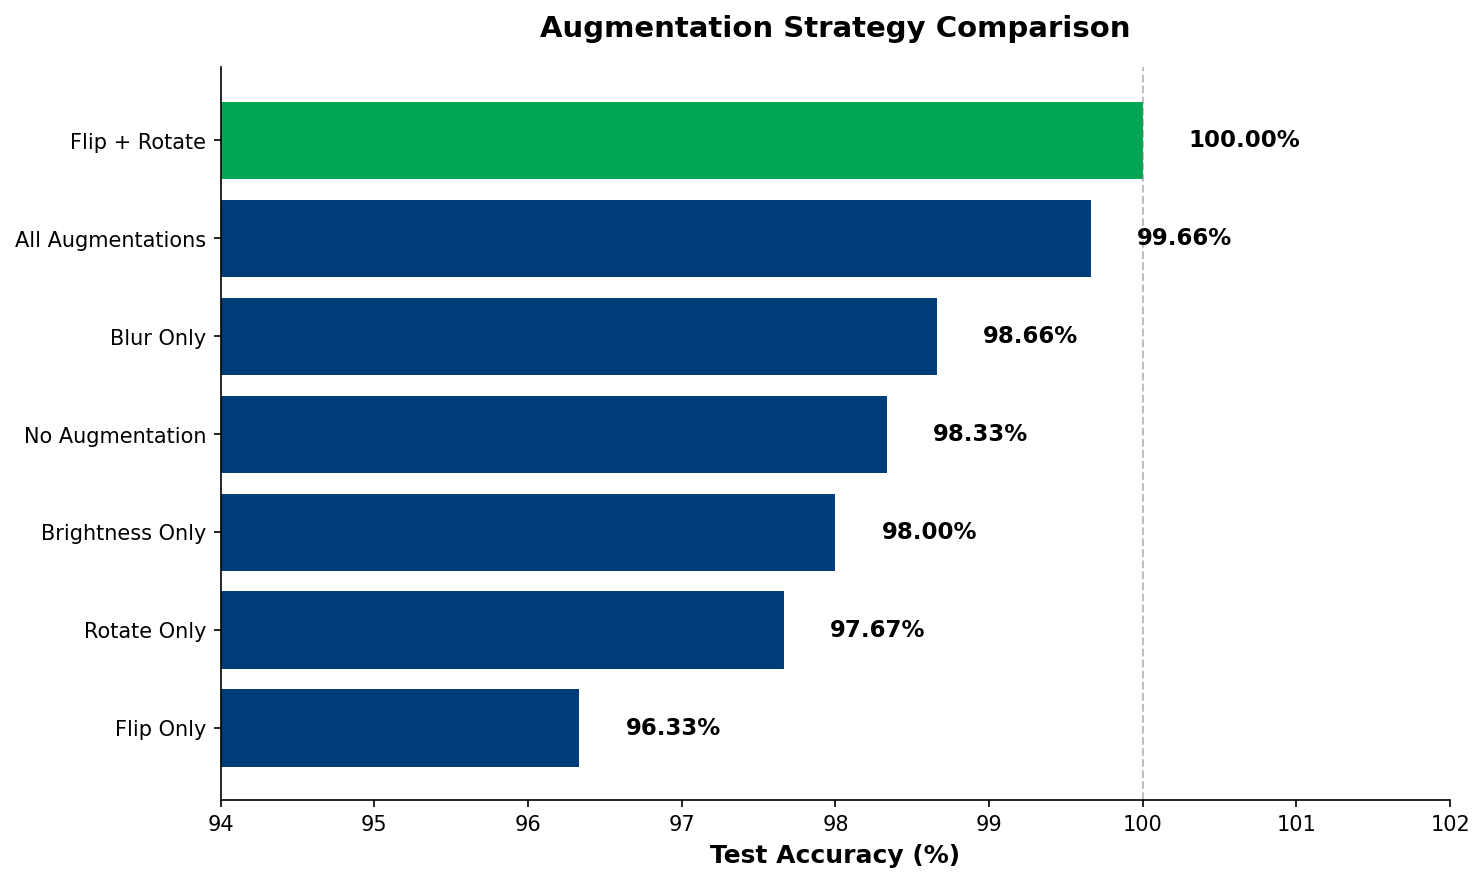
\includegraphics[width=\columnwidth]{images/augmentation_comparison.png}
    \caption{Test accuracy comparison across augmentation strategies. Flip+rotate achieves 100\% accuracy.}
    \label{fig:aug_comparison}
\end{figure}

Figure~\ref{fig:conf_matrix} shows the confusion matrix for our best model (flip+rotate). No misclassifications.

\begin{figure}[H]
    \centering
    
\includegraphics[width=0.95\columnwidth]{images/confusion_matrix.png}
    \caption{Confusion matrix for flip+rotate model.}
    \label{fig:conf_matrix}
\end{figure}

\textbf{Dataset size results.} Table~\ref{tab:datasize} and Figure~\ref{fig:dataset_size} show that augmentation helps a lot when you have little data (90\% $\rightarrow$ 98\% with only 50 samples). With enough data, augmentation matters less.

\begin{table}[H]
\centering
\caption{Test accuracy by dataset size}
\label{tab:datasize}
\begin{tabular}{@{}lcc@{}}
\toprule
Samples/class & No Aug & With Aug \\
\midrule
50 & 90.00\% & 98.00\% \\
100 & 98.00\% & 97.00\% \\
200 & 99.00\% & 97.50\% \\
Full ($\sim$300) & 100.00\% & 99.67\% \\
\bottomrule
\end{tabular}
\end{table}

\begin{figure}[H]
    \centering
    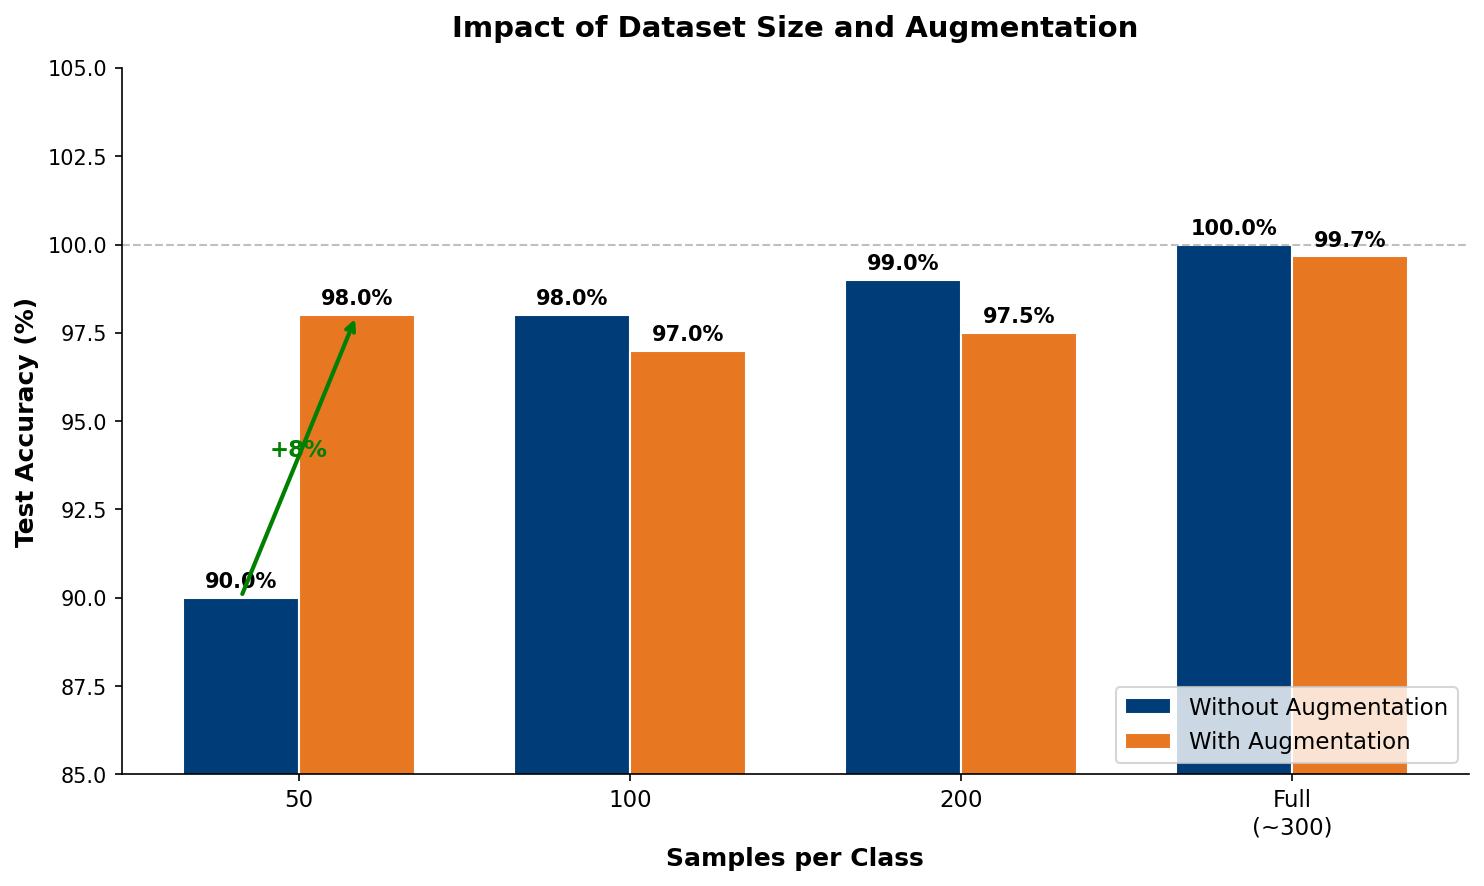
\includegraphics[width=\columnwidth]{images/dataset_size_effect.png}
    \caption{Impact of dataset size on accuracy. Augmentation provides an 8\% boost with only 50 samples per class.}
    \label{fig:dataset_size}
\end{figure}

\section*{Conclusion}
\textbf{What worked.} The biggest improvement came from adding hand cropping with MediaPipe. Before that, the model was basically useless. The flip+rotate augmentation combo worked best, probably because gestures can appear at different angles and orientations.

\textbf{What we struggled with.}
\begin{itemize}
    \item Initially had no idea why accuracy was bad -- turned out the model was learning backgrounds
    \item MediaPipe version issues (newer versions removed the API we needed, had to pin to 0.10.9)
    \item More augmentations didn't mean better results -- all augmentations actually performed slightly worse than just flip+rotate
\end{itemize}

\textbf{Limitations.}
\begin{itemize}
    \item Only 5 gestures
    \item Single hand only
    \item Needs decent lighting for MediaPipe to work
    \item Trained on our hands only -- might not generalize to other people
\end{itemize}

\end{document}
